\documentclass[twoside,12pt]{article}
\usepackage[left=1in, right=1in, top=1in, bottom=1in]{geometry}
\usepackage{amsmath}
\usepackage{amssymb}
\usepackage{amsfonts}
\usepackage{mathtools}
\usepackage{amsthm}
\usepackage{fancyhdr}
\usepackage{enumitem}
\usepackage{siunitx}
\usepackage{booktabs}
\usepackage[hidelinks]{hyperref}
\usepackage{sectsty}
\usepackage{mathrsfs} % mathscr
\usepackage{tikz}
\usepackage{pgfplots}
\usepackage{multicol}
\usepackage{listings}
% \usepackage{amsart}
\usepackage{fontspec}
\usepackage{titlesec}
\usepackage{subcaption}

% allow H option of figure
\usepackage{float}

% math font (libertine)
\usepackage{libertinus-otf}

% braket
\usepackage{braket}

% mono font
\usepackage{inconsolata}
\setmonofont{inconsolata}

% define Latin modern font environment
\newcommand{\lms}{\fontfamily{lmss}\selectfont} % Latin Modern Roman
% \newcommand{\lmss}{\fontfamily{lmss}\selectfont} % Latin Modern Sans
% \newcommand{\lmss}{\fontfamily{lmtt}\selectfont} % Latin Modern Mono

% % change mathcal shape
% \usepackage[mathcal]{eucal}


% define math operators
\newcommand{\FF}{\mathbb{F}}
\newcommand{\RR}{\mathbb{R}}
\newcommand{\NN}{\mathbb{N}}
\newcommand{\ZZ}{\mathbb{Z}}
\newcommand{\QQ}{\mathbb{Q}}
\newcommand{\XX}{\mathbb{Y}}
\newcommand{\CL}{\mathcal{L}}
% \renewcommand{\d}{\mathrm{d}}
\renewcommand*\d{\mathop{}\!\mathrm{d}}
\DeclareMathOperator*{\argmax}{arg\,max}
\DeclareMathOperator*{\argmin}{arg\,min}
\DeclareMathOperator{\im}{im}
\DeclareMathOperator{\id}{id}
\renewcommand{\mod}[1]{\ (\mathrm{mod}\ #1)}

% section font style
\sectionfont{\lms\large}
\subsectionfont{\lms\normalsize}
\subsubsectionfont{\bf}

% line spreading and break
\hyphenpenalty=5000
\tolerance=20
\setlength{\parindent}{0em}
\setlength\parskip{0.5em}
\allowdisplaybreaks
\linespread{0.9}

% theorem
% latex theorem
% definition style
\theoremstyle{definition}
\newtheorem{theorem}{Theorem}[subsection]
\newtheorem{axiom}{Axiom}[section]
\newtheorem{definition}{Definition}[section]
\newtheorem{example}{Example}[section]
\newtheorem{question}{Question}[section]
\newtheorem{exercise}{Exercise}[section]
\newtheorem*{exercise*}{Exercise}
\newtheorem{lemma}{Lemma}[section]
\newtheorem{proposition}{Proposition}[section]
\newtheorem{corollary}{Corollary}[section]
\newtheorem*{theorem*}{Theorem}
\newtheorem{problem}{Problem}
% remark style
\theoremstyle{remark}
\newtheorem*{remark}{Remark}
\newtheorem*{solution}{Solution}
\newtheorem*{claim}{Claim}


% paragraph indent
\setlength{\parindent}{0em}
\setlength\parskip{0.5em}

\newcommand\Code{CSC4005 FA22}
\newcommand\Ass{HW02}
\newcommand\name{Haoran Sun}
\newcommand\mail{haoransun@link.cuhk.edu.cn}

\title{{\lms \Code \ \Ass}}
\author{\lms \name \ (\href{mailto:\mail}{\mail})}
\date{\sffamily \today}

\makeatletter
% \let\Title\@title
\let\theauthor\@author
\let\thedate\@date

\fancypagestyle{plain}{%
    \fancyhf{}
    \lhead{\sffamily \Ass}
    \rhead{\sffamily \name}
    \rfoot{\sffamily\thepage}

    % # 页脚自定义
    \fancyfoot[L]{
        \begin{minipage}[c]{0.06\textwidth}
            
\includegraphics[height=7.5mm]{logo2.png}
        \end{minipage}
    }
}
\fancypagestyle{title}{%
    \fancyhf{}
    \renewcommand{\headrulewidth}{0pt}
    % \lhead{\Title}
    % \rhead{\theauthor}
    \rfoot{\sffamily\thepage}

    % # 页脚自定义
    \fancyfoot[L]{
        \begin{minipage}[c]{0.06\textwidth}
            
\includegraphics[height=7.5mm]{logo2.png}
        \end{minipage}
    }
}
\fancyfootoffset[L]{0.3cm}

% re-define title format
\makeatletter
\renewcommand{\maketitle}{\bgroup\setlength{\parindent}{0pt}
\begin{flushleft}
  \textbf{\Large\@title}

  \@author
\end{flushleft}\egroup
}
\makeatother

\pagestyle{plain}

% lstlisting settings
\lstset{
    basicstyle=\linespread{0.8}\ttfamily\small,
    breaklines=true,
    basewidth=0.5em,
    frame=single,
}
\lstdefinestyle{output}{
    basicstyle=\linespread{0.8}\ttfamily\footnotesize,
    breaklines=true,
    basewidth=0.5em,
    frame=single,
}    
\lstdefinestyle{sh}{
    basicstyle=\linespread{0.8}\ttfamily\footnotesize,
}
\lstdefinestyle{cpp}{
    numbers=left,
    basicstyle=\linespread{0.8}\ttfamily\footnotesize,
    numberstyle=\linespread{0.8}\ttfamily\footnotesize,
    language=C++,
    xleftmargin=6.0ex,
    frame=single,
}


\begin{document}
\maketitle
\thispagestyle{title}

\section{Introduction}
The Mandelbrot set is the set of complex numbers $c\in\mathbb{C}$ that does not diverges
under the following iteration, start from $z_0 = c$.
\begin{align}
    z_{n+1}^2 = z^2 + c
    \label{eq:manditer}
\end{align}
The set can be visualized through numerical computation.
By setting a rectangular region (should be aligned to the real and imaginary axis) 
in the complex plane, one can divide it into a mesh of points.
Setting a maximum iteration number $m_\text{max}$ and then perform iteration 
on each point using the equation \ref{eq:manditer} until it diverges.
Let $m(c)$ be the number of iteration steps that the point diverges, then
$m(c)/m_\text{max}$ could be an estimator of the density of Mandelbrot set
around this point.
Then, the density of Mandelbrot set could be visualized according to $m(c)$ and $m_\text{max}$.

However, the computation is intensive.
Suppose we are going to obtain an image with resolution $m\times n$,
the computational complexity would be $O(nm)$.
In order to accelerate the computation, in this assignment, two parallel scheme
are implemented: MPI and Pthread.
Programs are tested under different resolutions and numbers of CPU cores.
Speed-up factor and CPU efficiency are also analyzed.




\section{Method}
\subsection{Program design and implementation}
All programs are implemented using C++ programming language.
MPICH and Pthreads are used for parallelism.
For visualization, OpenGL is used to implement a graphical render
while STB (single-file public domain libraries) is used to plot png images.

Please refer to Figure \ref{fig:mpiflow} for the MPI program flowchart and
Figure \ref{fig:pthflow} for the Pthreads program flowchart.
The sequential version were written in \lstinline|src/main.seq.cpp|,
MPI version \lstinline|src/main.mpi.cpp|,
Pthreads \lstinline|src/main.pthread.cpp|.


\subsection{Usage}
\textit{\color{red}
For convenience, one can directly execute 
demonstration shell scripts to have a first glimpse of the program.
One can refer to Figure \ref{fig:demo} for sample GUI output.
}
\begin{lstlisting}[style=sh]
cd hw02
./scripts/demo.seq.sh
./scripts/demo.mpi.sh
./scripts/demo.pthread.sh
./scripts/demo.pthread_ds.sh # ds means dynamic scheduling
\end{lstlisting}

The program is compiled using CMake build system.
One can have a look at \lstinline|CMakeLists.txt| and \lstinline|src/CMakeLists.txt| 
to check compilation requirements.
If one wants to build the program with the GUI feature, he can run the following commands to
configure and start compilation under \lstinline|hw02| directory.
To disable the GUI feature, one can set \lstinline|-DGUI=OFF| in the configure process.
The compiled programs would be placed in \lstinline|build/bin| directory.
\begin{lstlisting}[style=sh]
cmake -B build -DCMAKE_BUILD_TYPE=Release -DGUI=ON
cmake --build build
\end{lstlisting}

One can run the program using the following commands,
where \lstinline|xmax|, \lstinline|xmin|, \lstinline|ymax|, \lstinline|ymin|
set the range of the rectangular region in the complex plane;
\lstinline|ndim| sets the resolution (partition of the mesh) on
$x$-direction (real line);
\lstinline|record| determines whether the runtime data would be saved;
\lstinline|save| controls if the image would be saved.
After executing the program,
a GUI window should be prompted to display the density
and an image \lstinline|mandelbrot_$jobtype.png| similar to 
Figure \ref{fig:image} would be saved.
\begin{lstlisting}[style=sh]
paras="--ndim 2000 --xmin -0.125 --xmax 0.125 --ymin 0.6 --ymax 0.7"
record="--record 0"
save="--save 1"
./build/bin/main.seq $paras $save $record               # sequential program
mpirun -np 4 ./build/bin/main.mpi $paras $save $record  # mpi program   
./build/bin/main.pthread    -nt 4 $paras $save $record  # pthreads program
./build/bin/main.pthread_ds -nt 4 $paras $save $record  # dynamic scheduling pthreads program 
\end{lstlisting}
\begin{figure}[h!]
    \centering
    \includegraphics[width=\textwidth]{../mandelbrot_pth.png}
    \caption{Sample output image}
    \label{fig:image}
\end{figure}

\subsection{Performance evaluation}
In order to evaluate the parallel code, the program was executed under 
different configurations.
With 20 different CPU core numbers (from 1 to 20 with increment 1, $p=1, 2,\dots, 20$)
and 20 different $x$-resolutions 
(from 500 to 10000 with increment 500, $n=500, 1000, \dots, 10000$), 
400 cases in total were sampled.
Recorded runtime and CPU time were analyzed through the Numpy
package in Python.
Figures were plotted through the Matplotlib and the Seaborn packages in Python.
Analysis code were written in \lstinline|analysis/main.ipynb|.

\newpage
\section{Result and Discussion}
\subsection{Runtime}
\begin{figure}[t!]
    \centering
    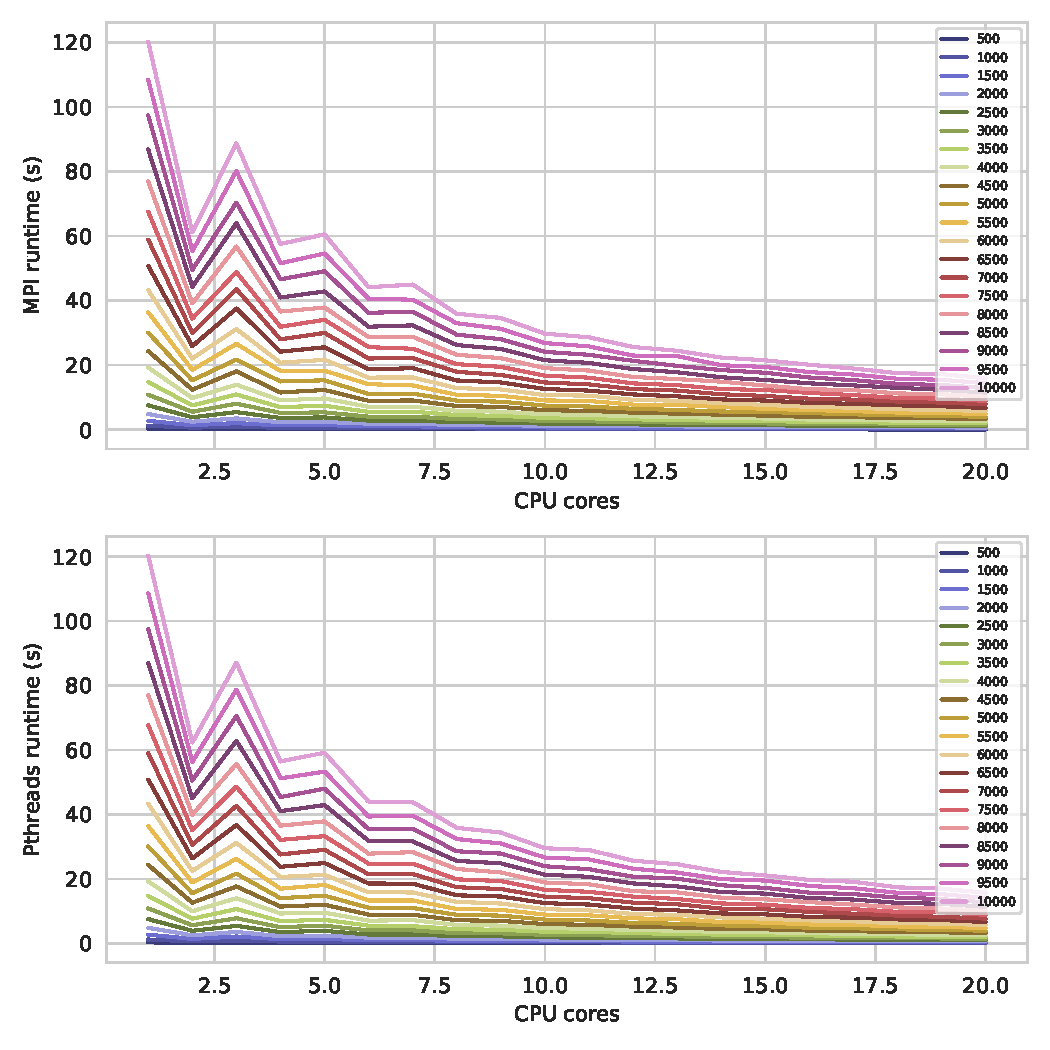
\includegraphics[width=\textwidth]{../analysis/runtime-core.pdf}
    \caption{Runtime vs CPU cores plot.}
    \label{fig:runtime-core}
\end{figure}

\begin{figure}[t!]
    \centering
    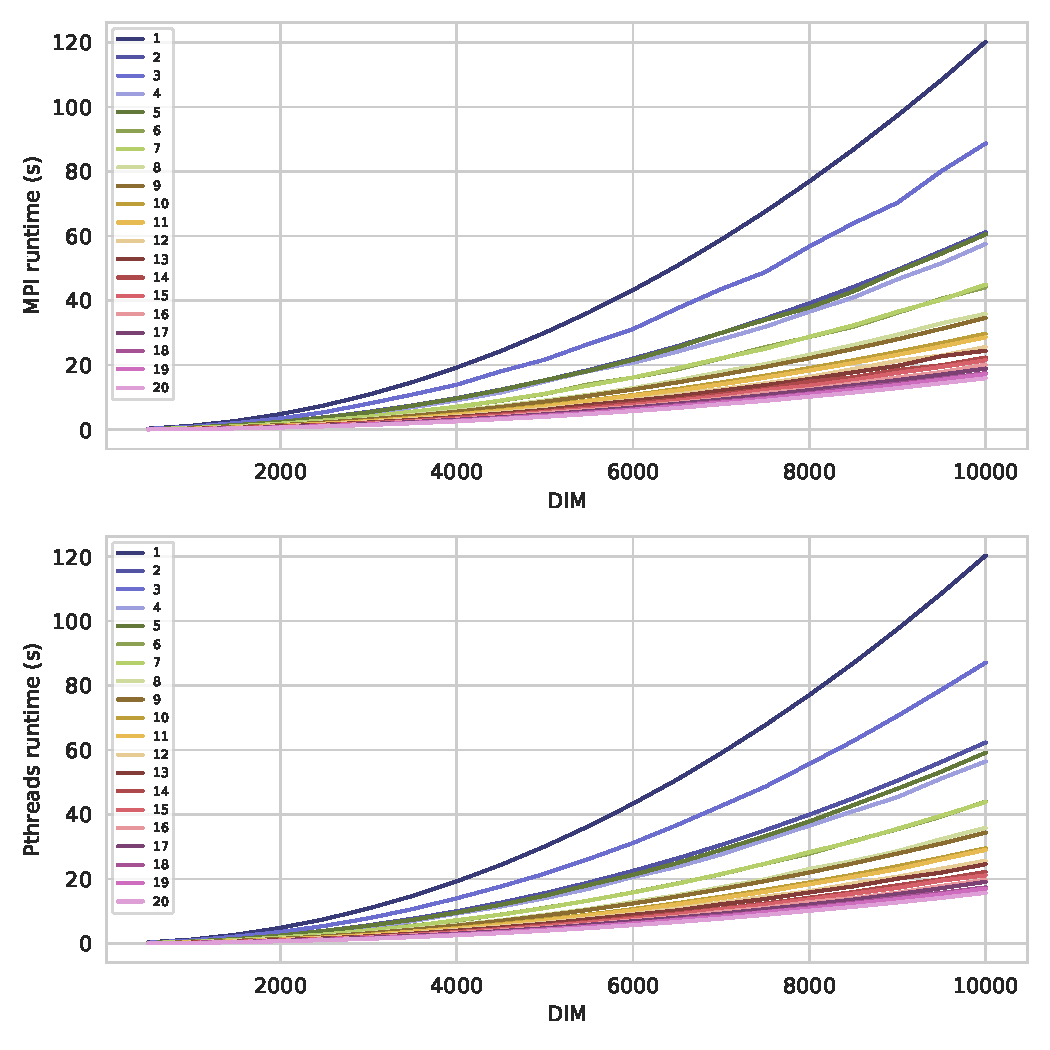
\includegraphics[width=\textwidth]{../analysis/runtime-dim.pdf}
    \caption{Runtime vs $x$-resolution plot.}
    \label{fig:runtime-dim}
\end{figure}

The graph of running time versus CPU cores and versus array size were plotted
in Figure \ref{fig:runtime-core} and \ref{fig:runtime-dim}, respectively.
From Figure \ref{fig:runtime-dim}, the plot clearly shows a perfect $O(n^2)$
the complexity of the algorithm, which is consistent with the theoretical analysis.
From figure \ref{fig:runtime-core}, however, for a fixed array size, 
the runtime does not monotonically decrease with the increase of CPU cores.
It shows a zig-zag pattern from CPU cores ranging from 1 to 7.
The reason behind this is the static scheduling algorithm used in the
parallel program.
According to the flowchart in Figure \ref{fig:mpiflow} and \ref{fig:pthflow},
the mesh is averagely distributed to each process/thread.
Nevertheless, the computation time of each thread may not be the same,
which means some thread may finish their job very fast and keep waiting
other threads finish their job. 
This issue would be further discussed in the following sections.

Due to the static scheduling algorithm, the performance of 
MPI and Pthreads are approximately the same, as Figure \ref{fig:mpiflow}
shown.


\clearpage
\newpage
\subsection{Performance analysis}
The heatmap of acceleration is plotted in Figure \ref{fig:heatmap-rate}.
It should be noticed that when the array size is large ($n\geq 1000$), 
the speed-up ratio does not change a lot,
which means the time spent on communication (MPI) and
shared-memory operations (Pthreads) are comparatively 
a small part of the overall execution time.
Moreover, from the first row of the heatmaps,
the acceleration rate of Pthread is relatively lower than
MPI's speed-up ratio, which indicates the creation and joining
of threads could be time-consuming.

\begin{figure}[h!]
    \centering
    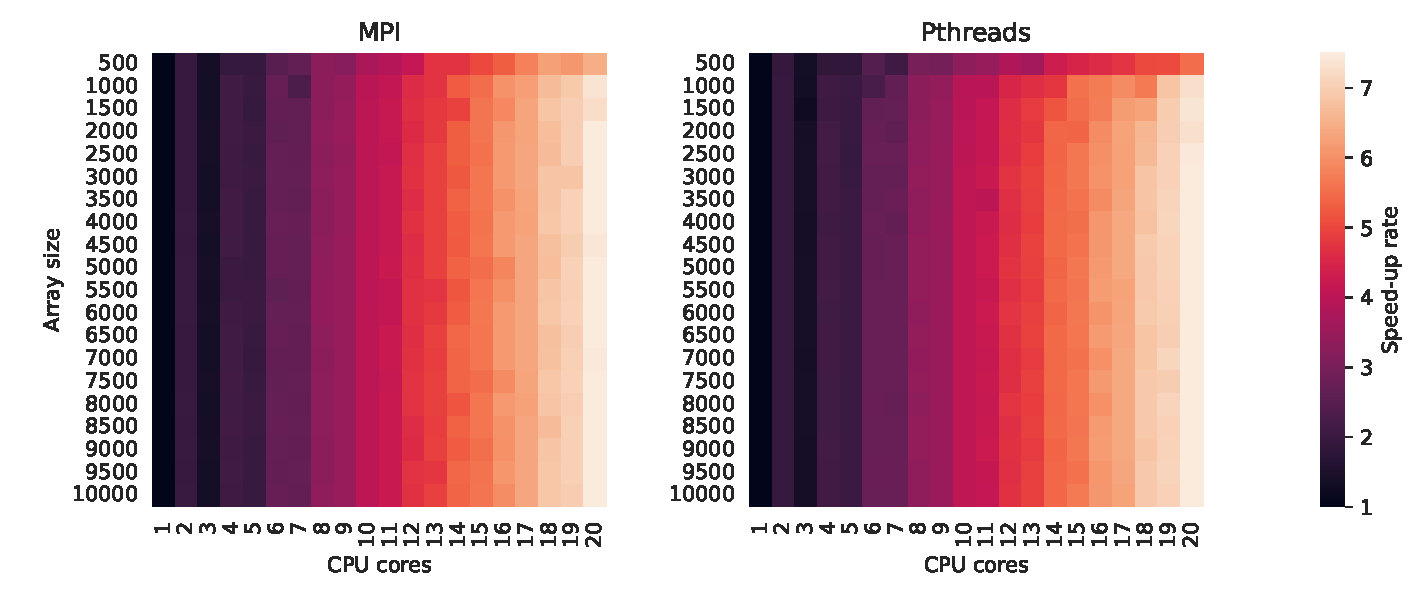
\includegraphics[width=\textwidth]{../analysis/heatmap-rate.pdf}
    \caption{Speed-up ratio of two parallel programs.}
    \label{fig:heatmap-rate}
\end{figure}
\begin{figure}[h!]
    \centering
    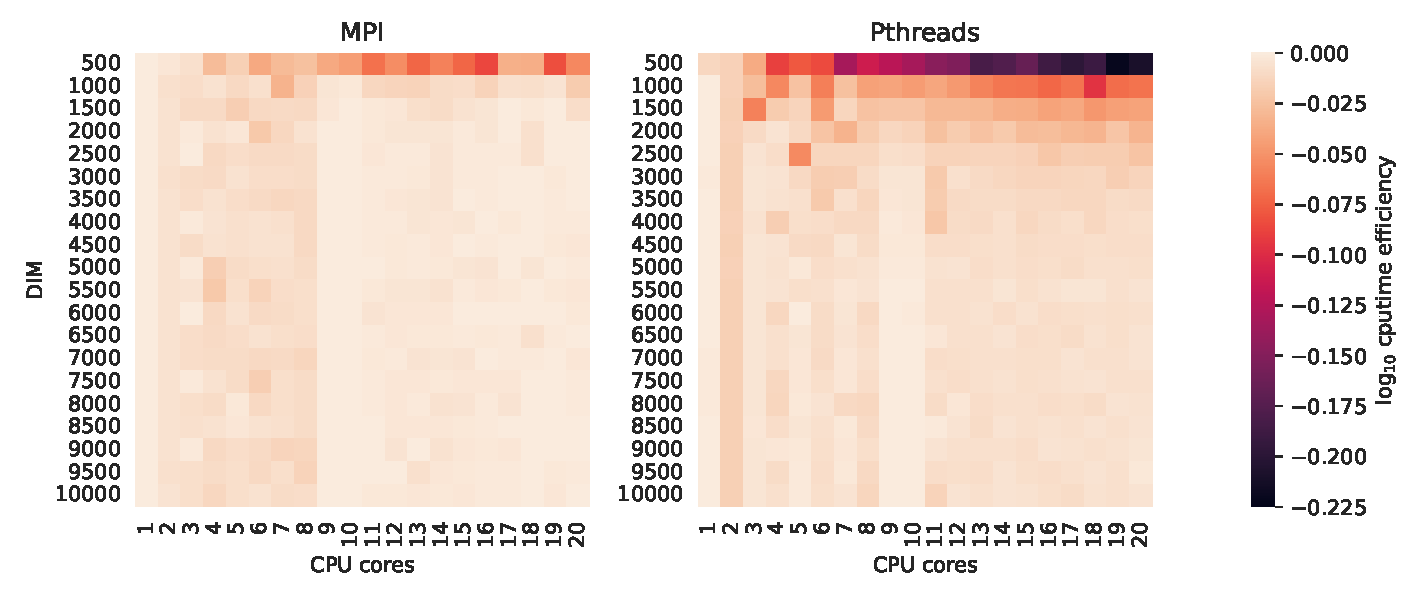
\includegraphics[width=\textwidth]{../analysis/heatmap-cpueff.pdf}
    \caption{$\log_10$ CPU time efficiency.}
    \label{fig:heatmap-cpueff}
\end{figure}

The heatmap of CPU time spent on computation is plotted in
Figure \ref{fig:heatmap-cpueff}.
It should be clear that when the array size is large, 
the computation efficiency of the parallel program
is the same as the computational efficiency of the sequential program.
Then, we can again confirm that the relative-low efficiency
of the parallel program is caused by the scheduling algorithm
which performs partition. 

To solve this issue, one may apply \textbf{dynamic scheduling}.
The dynamic scheduling would constantly check the status of each process/thread
and utilize spare computational resources dynamically and efficiently.
For example, the dynamic scheduling scheme in this homework is completed by
set several variables: \lstinline|max_idx| is the number of total jobs,
\lstinline|curr_idx| records how many jobs have been finished, 
\lstinline|jobsize| is the data points that each process will process in 
one iteration.
In each iteration, the thread will first check if there are unfinished
jobs. If there is, a computing job with a size equal to \lstinline|jobsize|
will be assigned to this thread.
If not, the program will terminate the calculation.
In this case, \lstinline|jobsize| is set to be 500*500.
Note that Pthreads mutex lock is useful to avoid racing problems.
One can refer to \lstinline|src/main.pthread_ds.cpp| and
\lstinline|mandelbrot_loop_pt_ds| in \lstinline|src/utils.h| for detailed implementation.
Dynamic scheduling is useful when the problem size is large.
As Figure \ref{fig:ds} shown, in the Pthreads implementation of dynamic
scheduling, it can further speed up the naive Pthreads
calculation up to more than 2.5 times.

\begin{figure}[h!]
    \centering
    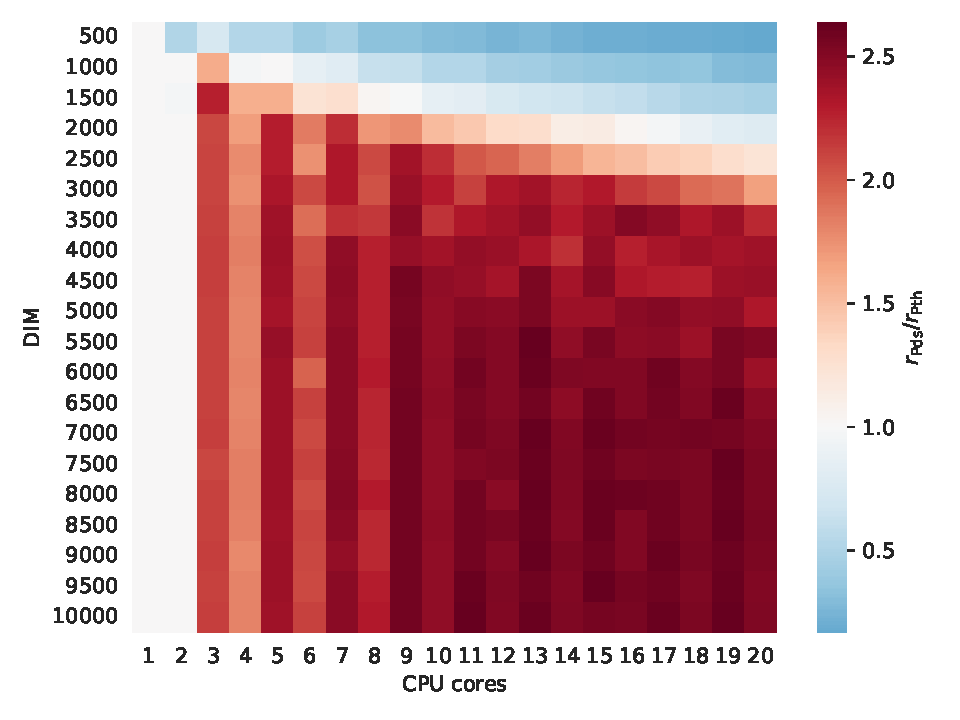
\includegraphics[width=\textwidth]{../analysis/pds2pth.pdf}
    \caption{Dynamic scheduling speed up vs naive parallel speed-up}
    \label{fig:ds}
\end{figure}




\section{Conclusion}
In conclusion, two parallel computing schemes for Mandelbrot set were implemented and
their performances were compared and evaluated.
One should use dynamic scheduling when dealing with large-scale computations
to fully utilize computational resources.

\appendix
% \renewcommand\thefigure{\thesection.\arabic{figure}}
\counterwithin{figure}{section}

\newpage
\section{Supplementary figures}
\begin{figure}[h!]
    \centering
    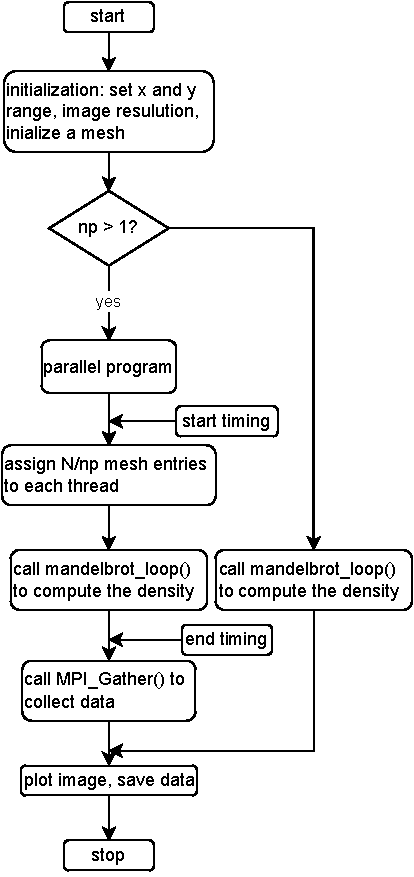
\includegraphics[scale=1.35]{../flowchart_mpi.drawio.pdf}
    \caption{MPI program flowchart}
    \label{fig:mpiflow}
\end{figure}

\begin{figure}[h!]
    \centering
    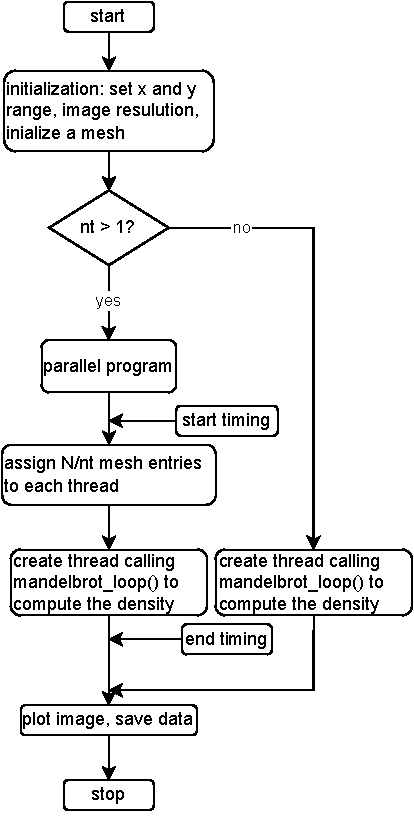
\includegraphics[scale=1.35]{../flowchart_pthread.drawio.pdf}
    \caption{Pthreads program flowchart}
    \label{fig:pthflow}
\end{figure}

\begin{figure}[h!]
    \centering
    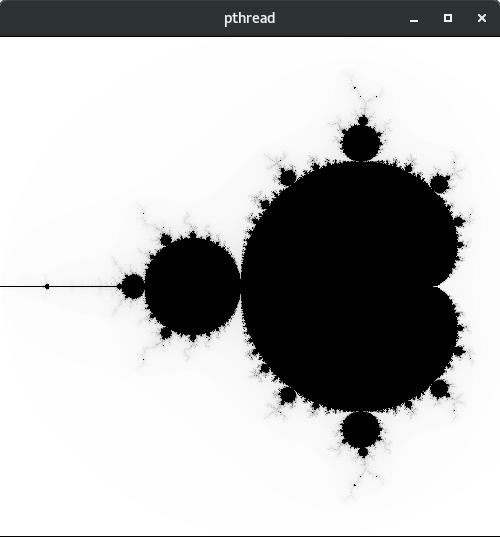
\includegraphics[width=0.6\textwidth]{../demo.png}
    \caption{Sample GUI output by executing \lstinline|scripts/demo.pthread.sh|.}
    \label{fig:demo}
\end{figure}

\begin{figure}[h!]
    \centering
    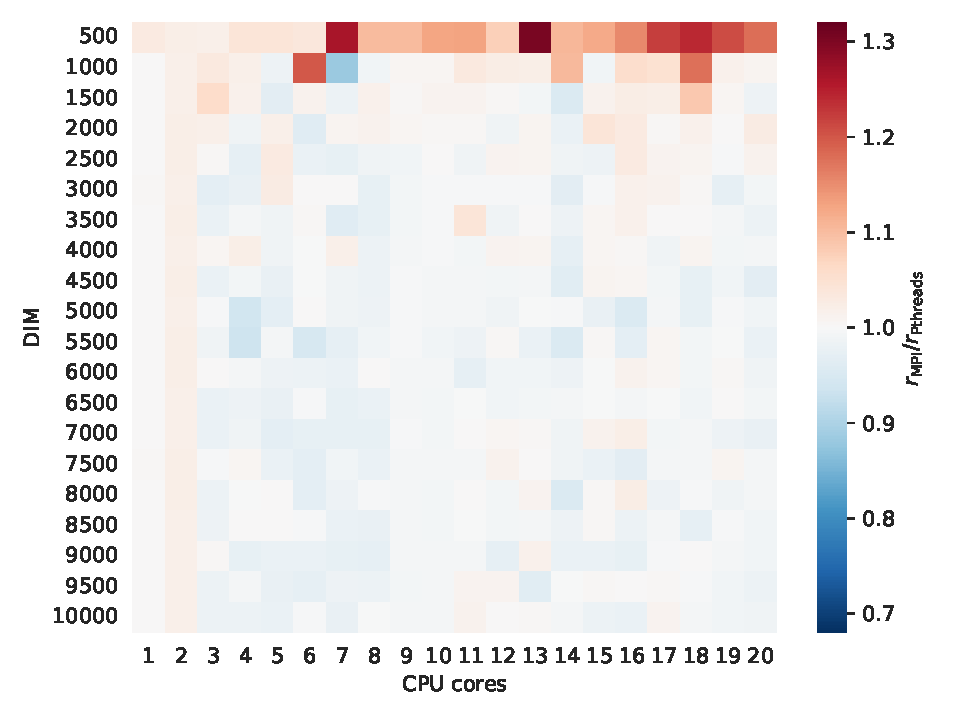
\includegraphics[width=0.7\textwidth]{../analysis/mpi2pth.pdf}
    \caption{Ratio of MPI and Pthreads speed-up rate.}
    \label{fig:mpi2pth}
\end{figure}

\clearpage
\newpage
\section{Source code}
\lstinputlisting[style=cpp,language=,title=\lstinline|CMakeLists.txt|]{../CMakeLists.txt}
\lstinputlisting[style=cpp,language=,title=\lstinline|src/CMakeLists.txt|]{../src/CMakeLists.txt}
\lstinputlisting[style=cpp,title=\lstinline|src/main.seq.cpp|]{../src/main.seq.cpp}
\lstinputlisting[style=cpp,title=\lstinline|src/main.mpi.cpp|]{../src/main.mpi.cpp}
\lstinputlisting[style=cpp,title=\lstinline|src/main.pthread.cpp|]{../src/main.pthread.cpp}
\lstinputlisting[style=cpp,title=\lstinline|src/utils.h|]{../src/utils.h}





% \end{multicols*}
\end{document}

